\documentclass{article}

\usepackage{tikz} 
\usetikzlibrary{automata, positioning, arrows} 

\usepackage{amsthm}
\usepackage{amsfonts}
\usepackage{amsmath}
\usepackage{amssymb}
\usepackage{fullpage}
\usepackage{color}
\usepackage{parskip}
\usepackage{hyperref}
  \hypersetup{
    colorlinks = true,
    urlcolor = blue,       % color of external links using \href
    linkcolor= blue,       % color of internal links 
    citecolor= blue,       % color of links to bibliography
    filecolor= blue,        % color of file links
    }
    
\usepackage{listings}

\definecolor{dkgreen}{rgb}{0,0.6,0}
\definecolor{gray}{rgb}{0.5,0.5,0.5}
\definecolor{mauve}{rgb}{0.58,0,0.82}

\lstset{frame=tb,
  language=haskell,
  aboveskip=3mm,
  belowskip=3mm,
  showstringspaces=false,
  columns=flexible,
  basicstyle={\small\ttfamily},
  numbers=none,
  numberstyle=\tiny\color{gray},
  keywordstyle=\color{blue},
  commentstyle=\color{dkgreen},
  stringstyle=\color{mauve},
  breaklines=true,
  breakatwhitespace=true,
  tabsize=3
}

\newtheoremstyle{theorem}
  {\topsep}   % ABOVESPACE
  {\topsep}   % BELOWSPACE
  {\itshape\/}  % BODYFONT
  {0pt}       % INDENT (empty value is the same as 0pt)
  {\bfseries} % HEADFONT
  {.}         % HEADPUNCT
  {5pt plus 1pt minus 1pt} % HEADSPACE
  {}          % CUSTOM-HEAD-SPEC
\theoremstyle{theorem} 
   \newtheorem{theorem}{Theorem}[section]
   \newtheorem{corollary}[theorem]{Corollary}
   \newtheorem{lemma}[theorem]{Lemma}
   \newtheorem{proposition}[theorem]{Proposition}
\theoremstyle{definition}
   \newtheorem{definition}[theorem]{Definition}
   \newtheorem{example}[theorem]{Example}
\theoremstyle{remark}    
  \newtheorem{remark}[theorem]{Remark}

\setcounter{tocdepth}{3}  % This makes subsubsections (level 3) appear in TOC
\setcounter{secnumdepth}{3}  % This makes subsubsections numbered
  

\title{CPSC-406 Report}
\author{Shuntaro Abe  \\ Chapman University}

\date{\today} 

\begin{document}

\maketitle

\begin{abstract}
This is the place to write an abstract. The abstract should be a short summary of the report. It should be written in a way that makes it possible to understand the purpose of the report without reading it. You can write a dummy abstract first and replace it with a real one later in the semester.
\end{abstract}

\setcounter{tocdepth}{3}
\tableofcontents

\section{Introduction}\label{intro}

Add introduction

\section{Week by Week}\label{homework}

\subsection{Week 1}


\subsubsection{Notes}

In Chapter 2.1 of ITALC, we learn about regular languages, which are types of languages that can be described using finite automata. A finite automaton is a machine that has a set of states, and it changes between these states based on input it receives. These machines are divided into two types: deterministic and nondeterministic.

In a deterministic finite automaton (DFA), the machine is always in one state at a time, while in a nondeterministic finite automaton (NFA), the machine can be in multiple states at once. Even though NFAs can be more flexible in how they process information, they don’t allow us to define any languages that a DFA can’t. However, NFAs can be more efficient and easier to describe certain problems, and later on, we can convert them into DFAs.

Additionally, the chapter introduces an extended form of NFA that can make transitions without any input. These types of automata are probably important when we later study regular expressions, as they are equivalent in the languages they can define.


\subsubsection{Homework}

We are given a parking machine that accepts 5 cent and 10 cent coins and needs to reach a total of 25 cents. The goal is to describe the automaton for this machine, identify the transitions between states, and characterize all the accepted words (i.e., the sequences of 5-cent and 10-cent coins that sum to 25 cents). Additionally, express the accepted words as a regular expression.

\textbf{Solution:}



\begin{itemize}
    \item The initial state is state 0.
    \item The final (accepting) state is state 25.
    \item Transitions from each state:
    \begin{itemize}
        \item From state 0, a 5 cents moves the machine to state 5.
        \item From state 0, a 10 cents moves the machine to state 10.
        \item From state 5, a 5 cents moves the machine to state 10.
        \item From state 5, a 10cents moves the machine to state 15.
        \item From state 10, a 5 cents moves the machine to state 15.
        \item From state 10, a 10 cents moves the machine to state 20.
        \item From state 15, a 5 cents moves the machine to state 20.
        \item From state 15, a 10 cents moves the machine to state 25 (accepting state).
        \item From state 20, a 5 cents moves the machine to state 25 (accepting state).
    \end{itemize}
\end{itemize}


Automaton visualized:

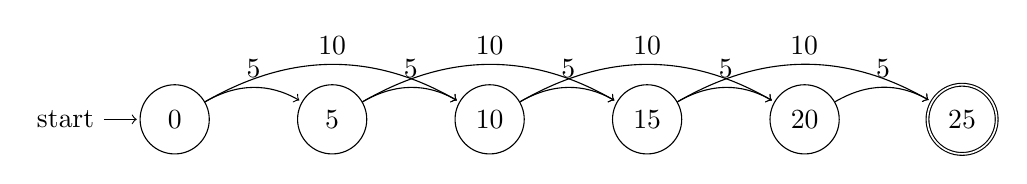
\begin{tikzpicture}[shorten >=1pt,node distance=2cm,on grid,auto] 
  % Define states in a straight line
  \node[state, initial] (q_0)   {$0$};  % q0 is the start state
  \node[state] (q_5) [right=of q_0] {$5$}; 
  \node[state] (q_10) [right=of q_5] {$10$};
  \node[state] (q_15) [right=of q_10] {$15$};
  \node[state] (q_20) [right=of q_15] {$20$};
  \node[state, accepting] (q_25) [right=of q_20] {$25$};  % q25 is the final state

  % Define transitions with curved arrows for inputs 5 and 10
  \path[->] 
    (q_0) edge [bend left] node {5} (q_5)      % From state 0 to state 5 with input 5
          edge [bend left] node {10} (q_10)    % From state 0 to state 10 with input 10
    (q_5) edge [bend left] node {5} (q_10)     % From state 5 to state 10 with input 5
          edge [bend left] node {10} (q_15)    % From state 5 to state 15 with input 10
    (q_10) edge [bend left] node {5} (q_15)    % From state 10 to state 15 with input 5
           edge [bend left] node {10} (q_20)    % From state 10 to state 20 with input 10
    (q_15) edge [bend left] node {5} (q_20)    % From state 15 to state 20 with input 5
           edge [bend left] node {10} (q_25)   % From state 15 to state 25 with input 10
    (q_20) edge [bend left] node {5} (q_25);   % From state 20 to state 25 with input 5
\end{tikzpicture}



To characterize the accepted words, we need to find all valid combinations of 5 cent and 10 cent coins that add up to 25. The valid combinations of coins are:

\[
\begin{aligned}
    5, 5, 5, 5, 5, \\
    5, 10, 5, 5, 5, \\
    10, 5, 10, 5, \\
    10, 10, 5, \\
    5, 10, 10, 5, \\
\end{aligned}
\]


Meaning that the accepted words are all of the possible combinations that end up at 25.

Regular Expression:

We can express the accepted words using a regular expression that describes the valid sequences of 5 cent and 10 cent coins. The regular expression for this automaton is:

\[
(5 \cdot 5 \cdot 5 \cdot 5 \cdot 5) \mid (5 \cdot 10 \cdot 5 \cdot 5 \cdot 5) \mid (10 \cdot 5 \cdot 10 \cdot 5) \mid (10 \cdot 10 \cdot 5) \mid (5 \cdot 10 \cdot 10 \cdot 5)
\]

This regular expression includes all of the possible combinations to get to 25 cents.


\subsubsection{Exploration}

The study of regular languages and finite automata is essential for understanding how machines process languages and information. It introduces key concepts in computer science such as how we can represent complex patterns in data using simple states and transitions. This material connects to broader themes in computation, such as parsing, compilers, and artificial intelligence, where automata theory helps model and solve problems efficiently. By understanding regular languages, we gain tools to describe and analyze computational problems in a structured way, making it a foundational topic for both theoretical and practical applications.


\subsubsection{Questions}

What role do empty string transitions play in regular languages, and how do they affect the design of automata or regular expressions?

\subsection{Week 2}

\subsubsection{Notes}

This week, we moved from the informal idea that a DFA accepts a string if it ends in an accepting state, to a more formal definition using the concept of an extended transition function.

The extended transition function, usually written as $\hat{\delta}$, tells us what state the DFA will be in after processing an entire string, not just one symbol. It's defined using induction:

- For the empty string, the DFA stays in the same state.
- For any non-empty string, we break the string into two parts: all but the last symbol (called $x$), and the last symbol (called $a$). We first compute the state reached after processing $x$, and then follow the transition on $a$ from that state.

This function is important because it gives a precise definition for what it means for a DFA to accept a string. A DFA accepts a string $w$ if $\hat{\delta}(q_0, w)$ is in the set of accepting states.

We also saw how this idea is directly used in the implementation of the \texttt{run} method in Python, which updates the state one symbol at a time while reading the input string.


\subsubsection{Homework}

\textbf{Exercise 2: Implementing DFA Runs}

\textit{Problem:}  
Download the lab source files. Navigate to \texttt{dfa.py}. Implement the \texttt{run} method.  
In the file \texttt{dfa\_ex01.py}, define the DFAs $A_1$ and $A_2$ from above.  
Test the correctness of your implementation by running \texttt{dfa\_ex01.py}.  
Add additional words to test your implementation and hypotheses from above.

\vspace{0.5em}

\textbf{Solution:}

The \texttt{run} method was implemented to simulate the execution of a deterministic finite automaton (DFA) on a given input string. It initializes the current state to the start state and then processes each symbol in the input one by one. For each symbol, it verifies that the symbol is valid for the DFA's alphabet and checks that a transition is defined. It then updates the current state based on the transition function. After consuming the entire input, the method returns \texttt{True} if the final state is an accepting state, and \texttt{False} otherwise.

\begin{lstlisting}[language=Python]
def run(self, w):
    current_state = self.q0
    for symbol in w:
        if symbol not in self.Sigma:
            return False
        if (current_state, symbol) not in self.delta:
            return False
        current_state = self.delta[(current_state, symbol)]
    return current_state in self.F
\end{lstlisting}

Next, I instantiated two DFAs in \texttt{dfa\_ex01.py} and tested them on all 3-letter words over the alphabet \texttt{\{a, b\}}:

\begin{lstlisting}[language=Python]
import dfa

# generate words for testing
def generate_words():
    words = []
    alphabet = ['a', 'b']
    for first in alphabet:
        for second in alphabet:
            for third in alphabet:
                words.append(first + second + third)
    return words

def __main__() :
    
    A1 = dfa.DFA(
        Q={1, 2, 3, 4},
        Sigma={'a', 'b'},
        delta={
            (1, 'a'): 2,
            (1, 'b'): 4,
            (2, 'a'): 2,
            (2, 'b'): 3,
            (3, 'a'): 3,
            (3, 'b'): 3,
            (4, 'a'): 4,
            (4, 'b'): 4
        },
        q0=1,
        F={3}
    )

    A2 = dfa.DFA(
        Q={1, 2, 3},
        Sigma={'a', 'b'},
        delta={
            (1, 'a'): 2,
            (1, 'b'): 1,
            (2, 'a'): 3,
            (2, 'b'): 1,
            (3, 'a'): 3,
            (3, 'b'): 1
        },
        q0=1,
        F={3}
    )

    words = generate_words()
    automata = [A1, A2]

    for X in automata:
         print(f"{X.__repr__()}")
         for w in words:
            print(f"{w}: {X.run(w)}")
         print("\n")

__main__()
\end{lstlisting}

\vspace{1em}

Both automata were tested successfully. The \texttt{run} method correctly simulates the transitions and final state checks, and the output matched the expected behavior based on each automaton's transition logic.


\textbf{Exercise 4: A New Automaton from an Old One}

\textit{Problem:}  
Consider the following automaton $A$:

Describe its accepted language $L(A)$.

On pen and paper, construct an automaton $A_0$ such that $A_0$ accepts exactly the words that $A$ refuses and vice versa.  
In \texttt{dfa.py}, implement the method \texttt{refuse} that takes in a DFA $A$ and returns a new DFA $A_0$ as above.  
Add $A$ and $A_0$ to \texttt{dfa\_ex03.py} and verify that \texttt{refuse} functions correctly by creating appropriate test cases.

\vspace{0.5em}

\textbf{Solution:}

\textit{Language Description:}  
The DFA $A$ accepts strings over $\{a, b\}$ that end in certain patterns depending on transitions to accepting states $q_2$ or $q_4$. From the structure, it accepts strings such as \texttt{a}, \texttt{b}, \texttt{ab}, etc., which lead to either of those states.

\vspace{0.5em}
\textit{DFA $A$ is shown below:}

\begin{center}
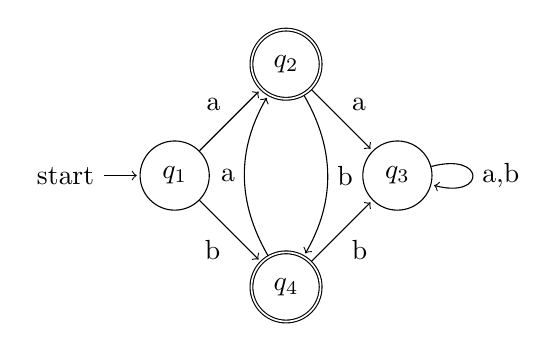
\begin{tikzpicture}[shorten >=1pt,node distance=2cm,on grid,auto]
  \node[state, initial] (q1) {$q_1$};
  \node[state, accepting] (q2) [above right=of q1] {$q_2$};
  \node[state] (q3) [below right=of q2] {$q_3$};
  \node[state, accepting] (q4) [below right=of q1] {$q_4$};

  \path[->]
    (q1) edge node {a} (q2)
         edge node [swap] {b} (q4)
    (q2) edge node {a} (q3)
         edge [bend left] node {b} (q4)
    (q3) edge [loop right] node {a,b} ()
    (q4) edge [bend left] node {a} (q2)
         edge node [swap] {b} (q3);
\end{tikzpicture}
\end{center}

\textit{DFA $A_0$ (the complement of $A$)} is constructed by making all non-accepting states into accepting states and vice versa. This results in the following automaton:

\begin{center}
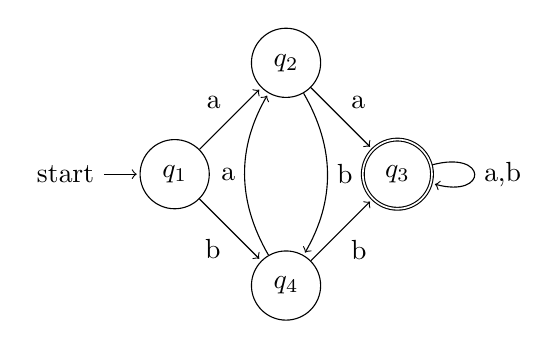
\begin{tikzpicture}[shorten >=1pt,node distance=2cm,on grid,auto]
  \node[state, initial] (q1) {$q_1$};
  \node[state] (q2) [above right=of q1] {$q_2$};
  \node[state, accepting] (q3) [below right=of q2] {$q_3$};
  \node[state] (q4) [below right=of q1] {$q_4$};

  \path[->]
    (q1) edge node {a} (q2)
         edge node [swap] {b} (q4)
    (q2) edge node {a} (q3)
         edge [bend left] node {b} (q4)
    (q3) edge [loop right] node {a,b} ()
    (q4) edge [bend left] node {a} (q2)
         edge node [swap] {b} (q3);
\end{tikzpicture}
\end{center}

\vspace{0.5em}
\textit{Implementation:}  
To construct the complement automaton programmatically, I added the following method to \texttt{dfa.py}:

\begin{lstlisting}[language=Python]
def refuse(self):
    new_F = self.Q - self.F  # Complement of accepting states
    return DFA(self.Q, self.Sigma, self.delta, self.q0, new_F)
\end{lstlisting}

I then added both $A$ and $A_0$ to \texttt{dfa\_ex03.py} and tested a range of words. I confirmed that for every word, $A$ accepts it if and only if $A_0$ rejects it, and vice versa.

This validates that the \texttt{refuse} function correctly generates the complement of a DFA.


\textbf{Exercise 2.2.4: Constructing DFAs}

\textit{Problem:}  
Give DFA’s accepting the following languages over the alphabet $\Sigma = \{0, 1\}$:

\begin{enumerate}
  \item The set of all strings ending in \texttt{00}.
  \item The set of all strings with three consecutive \texttt{0}s (not necessarily at the end).
  \item The set of strings with \texttt{011} as a substring.
\end{enumerate}

\vspace{1em}

\textbf{Solution:}

\begin{enumerate}

\item \textit{Strings ending in \texttt{00}}:

The DFA tracks the last two input symbols and accepts if they are both \texttt{0}.

\begin{center}
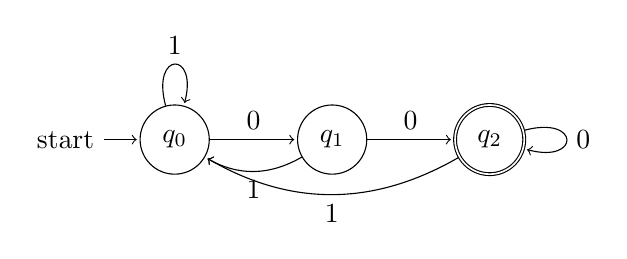
\begin{tikzpicture}[shorten >=1pt,node distance=2cm,on grid,auto]
  \node[state, initial] (q0) {$q_0$};
  \node[state] (q1) [right=of q0] {$q_1$};
  \node[state, accepting] (q2) [right=of q1] {$q_2$};

  \path[->]
    (q0) edge node {0} (q1)
         edge [loop above] node {1} ()
    (q1) edge node {0} (q2)
         edge [bend left] node {1} (q0)
    (q2) edge [loop right] node {0} ()
         edge [bend left] node {1} (q0);
\end{tikzpicture}
\end{center}


\item \textit{Strings with three consecutive \texttt{0}s}:

This DFA tracks up to three consecutive zeros and accepts once it sees \texttt{000}.

\begin{center}
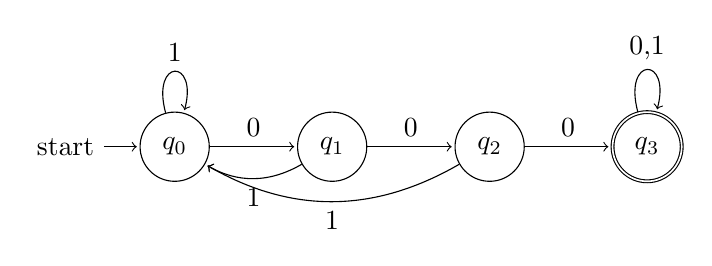
\begin{tikzpicture}[shorten >=1pt,node distance=2cm,on grid,auto]
  \node[state, initial] (q0) {$q_0$};
  \node[state] (q1) [right=of q0] {$q_1$};
  \node[state] (q2) [right=of q1] {$q_2$};
  \node[state, accepting] (q3) [right=of q2] {$q_3$};

  \path[->]
    (q0) edge node {0} (q1)
         edge [loop above] node {1} ()
    (q1) edge node {0} (q2)
         edge [bend left] node {1} (q0)
    (q2) edge node {0} (q3)
         edge [bend left] node {1} (q0)
    (q3) edge [loop above] node {0,1} ();
\end{tikzpicture}
\end{center}


\item \textit{Strings containing \texttt{011} as a substring}:

This DFA moves through a chain of states as it sees \texttt{0 → 01 → 011}.

\begin{center}
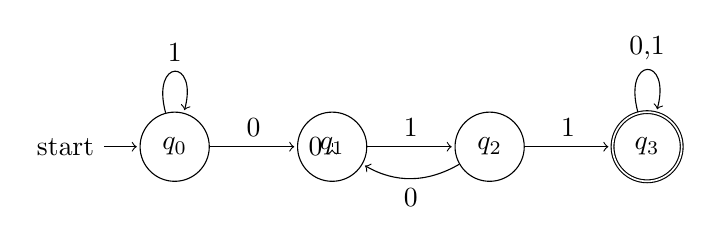
\begin{tikzpicture}[shorten >=1pt,node distance=2cm,on grid,auto]
  \node[state, initial] (q0) {$q_0$};
  \node[state] (q1) [right=of q0] {$q_1$};
  \node[state] (q2) [right=of q1] {$q_2$};
  \node[state, accepting] (q3) [right=of q2] {$q_3$};

  \path[->]
    (q0) edge node {0} (q1)
         edge [loop above] node {1} ()
    (q1) edge node {1} (q2)
         edge [bend left] node {0} (q1)
    (q2) edge node {1} (q3)
         edge [bend left] node {0} (q1)
    (q3) edge [loop above] node {0,1} ();
\end{tikzpicture}
\end{center}

\end{enumerate}

\subsubsection{Exploration}

The extended transition function gives us a solid foundation for thinking about what it really means for a DFA to accept a string. Instead of relying only on diagrams or intuition, we now have a way to describe DFA behavior using precise definitions.

This also connects well to programming. The way we defined $\hat{\delta}$ is almost the same as how we would write a function to simulate a DFA in code: start in a state, read each symbol in order, and move through the states based on the transition rules.

What makes this topic interesting is how it balances theory and practice. We’re learning how to think rigorously about something abstract — languages and automata — while also writing working code that simulates them. This foundation will help later when we study nondeterminism, minimization, and more advanced machines like pushdown automata and Turing machines.

\subsubsection{Questions}

What types of errors or edge cases can occur when simulating a DFA in code?

\subsection{Week 3}

\subsubsection{Notes}

This week we were introduced to nondeterministic finite automata (NFAs), which are an extension of deterministic finite automata (DFAs). The key idea behind an NFA is that it can be in multiple states at the same time — this is often interpreted as the machine having the ability to "guess" the correct path through its state transitions.

Instead of having a single unique transition from each state for each input symbol (as in a DFA), an NFA can have multiple possible transitions, or even no transition at all. This means that when an input symbol is read, the NFA can split into multiple possible computation paths.

Despite their different structure, NFAs are no more powerful than DFAs in terms of the languages they can recognize. Every NFA has an equivalent DFA that accepts the same language. However, the DFA equivalent can be significantly larger — in some cases, exponentially larger — than the original NFA.

NFAs are especially useful when designing automata for certain patterns or search tasks, such as recognizing keywords within long strings. Their structure tends to be simpler and more intuitive for complex language descriptions.

\subsubsection{Homework}

\textbf{Homework 1: Extended Transition Function}

We are given two DFAs, $A(1)$ and $A(2)$, over the alphabet $\Sigma = \{a, b\}$.

$L(A(1))$: The language of all non-empty strings where no two consecutive letters are the same.  
$L(A(2))$: The language of all strings of odd length such that every letter at an odd position is $a$.

\textit{Task 1: Compute } $\hat{\delta}_1(1, abaa)$

We simulate the transitions in $A(1)$ step by step:

\begin{itemize}
  \item Start at state 1
  \item Read $a$: move to state $q_a$
  \item Read $b$: move to state $q_b$
  \item Read $a$: move to state $q_a$
  \item Read $a$: transition fails (consecutive $a$'s not allowed), so the DFA rejects
\end{itemize}

Therefore, $\hat{\delta}_1(1, abaa)$ leads to a non-final or dead state.

\textit{Task 2: Compute } $\hat{\delta}_2(1, abba)$

We simulate the transitions in $A(2)$:

\begin{itemize}
  \item Length = 4 → even → may not be accepted
  \item 1st letter $a$ (odd position): OK
  \item 2nd letter $b$: OK
  \item 3rd letter $b$ (odd position): violates condition → not accepted
\end{itemize}

So $\hat{\delta}_2(1, abba)$ leads to a rejecting state.

\textbf{Homework 2: Product Automaton}

We want to construct a DFA $A$ such that $L(A) = L(A(1)) \cap L(A(2))$.

We use the definition of the product (or intersection) automaton:

\begin{itemize}
  \item $Q = Q(1) \times Q(2)$
  \item $\delta((q_1, q_2), a) = (\delta_1(q_1, a), \delta_2(q_2, a))$
  \item $q_0 = (q_0^{(1)}, q_0^{(2)})$
  \item $F = F(1) \times F(2)$
\end{itemize}

Each transition in the product DFA reflects the simultaneous transitions in both $A(1)$ and $A(2)$ under the same input. The product DFA accepts a string only if both original automata would accept it.

\textit{Why this works:} A string is accepted in the product DFA only if it ends in a state that is accepting in both $A(1)$ and $A(2)$. So this DFA precisely accepts the intersection of the two languages.

\textbf{Follow-up Question: Union Automaton}

To build a DFA $A'$ such that $L(A') = L(A(1)) \cup L(A(2))$, we again use the product DFA structure but change the set of accepting states:

\[
F' = (F(1) \times Q(2)) \cup (Q(1) \times F(2))
\]

This means that a string is accepted if it ends in a state that is accepting in \textit{either} $A(1)$ or $A(2)$ (or both).

This modification turns the product construction into a union construction instead of an intersection.


\subsubsection{Exploration}

One of the most interesting aspects of NFAs is how they offer a different perspective on computation. While DFAs model computation in a step-by-step, deterministic fashion, NFAs embrace uncertainty and parallelism. The idea that an automaton can explore many paths simultaneously is not just a mathematical trick — it's a powerful way to design algorithms that are more elegant and efficient to describe, even if they need to be "compiled down" to deterministic behavior in practice.

Another practical benefit is seen in pattern matching and regular expression engines. Many implementations are inspired by NFA-like behavior, where multiple paths are evaluated in parallel or lazily, to match patterns quickly and flexibly.

While NFAs do not expand the class of regular languages, they do highlight how representation and implementation can differ greatly even when the theoretical capability remains the same.


\subsubsection{Questions}

If an NFA can be in many states at once, does that mean it's faster than a DFA when used in real-world applications?

\subsection{Week 4}

\subsubsection{Notes}

\textbf{Section 3.1 – Regular Expressions:}

This section introduces regular expressions as a way to describe regular languages. Unlike automata, which are machine-like models, regular expressions use a symbolic language to describe patterns in strings. They are used in many software tools like \texttt{grep}, search functions in web browsers, and programs that help build compilers. A regular expression can represent the same languages as a deterministic or nondeterministic finite automaton. They are especially helpful because they are more readable and compact when expressing string patterns.

\textbf{Section 3.2.1 – Converting DFAs to Regular Expressions:}

This section explains how any deterministic finite automaton can be transformed into a regular expression that describes the same language. The process involves analyzing all the ways one can move from one state to another through the automaton without passing through certain other states. By building up from simple paths to more complex ones, we can eventually describe all possible paths in the automaton. This process is called \textit{state elimination} and leads to a regular expression that accepts the same strings as the original automaton.

\textbf{Section 3.2.2 – Completing the Construction:}

Here the method is extended to handle accepting states and loops. If the final state is the same as the start state, we add a loop to allow for repeated patterns. At the end, we combine all the possible ways to reach each accepting state to form one final regular expression. This expression will accept the same strings as the original automaton.

\subsubsection{Homework}

\textbf{Exercise 2:}

\textbf{Given DFA $A$:}

\begin{center}
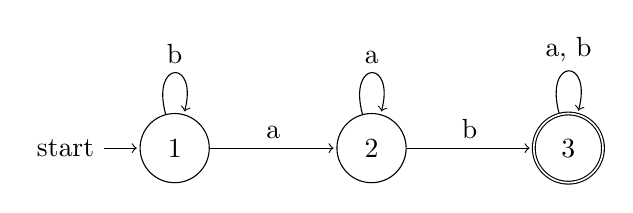
\begin{tikzpicture}[shorten >=1pt,node distance=2.5cm,on grid,auto]
  \node[state, initial] (q1) {$1$};
  \node[state] (q2) [right=of q1] {$2$};
  \node[state, accepting] (q3) [right=of q2] {$3$};

  \path[->] 
    (q1) edge [loop above] node {b} ()
         edge node {a} (q2)
    (q2) edge [loop above] node {a} ()
         edge node {b} (q3)
    (q3) edge [loop above] node {a, b} ();
\end{tikzpicture}
\end{center}

\textbf{1. Description of DFA $A$:}

\begin{itemize}
  \item $Q = \{1, 2, 3\}$ (states)
  \item $\Sigma = \{a, b\}$ (alphabet)
  \item $\delta$ (transition function):
  \[
  \begin{aligned}
  \delta(1, a) &= 2, &\delta(1, b) &= 1 \\
  \delta(2, a) &= 2, &\delta(2, b) &= 3 \\
  \delta(3, a) &= 3, &\delta(3, b) &= 3
  \end{aligned}
  \]
  \item $q_0 = 1$ (start state)
  \item $F = \{3\}$ (accepting state)
\end{itemize}

\textbf{2. Viewing DFA $A$ as an NFA:}

Any DFA can be understood as a special case of an NFA. In a DFA, the transition function is:
\[
\delta: Q \times \Sigma \rightarrow Q
\]
In an NFA, the transition function is:
\[
\delta': Q \times \Sigma \rightarrow \mathcal{P}(Q)
\]
We can define the NFA $A'$ equivalent to DFA $A$ as follows:
\[
A' = (Q, \Sigma, \delta', q_0, F)
\]
Where:
\[
\delta'(q, a) = \{\delta(q, a)\} \quad \text{for all } q \in Q, a \in \Sigma
\]

This interpretation means that every DFA is trivially an NFA where each input leads to exactly one state. Therefore, no nondeterminism is introduced, and the language accepted by $A'$ is exactly the same as the one accepted by $A$:
\[
L(A) = L(A')
\]

\textbf{3. Justification:}

The construction preserves the language because:
\begin{itemize}
  \item The same start and accepting states are used.
  \item The transition function returns singleton sets, introducing no extra nondeterminism.
  \item The paths through the automaton remain unchanged.
\end{itemize}

Thus, this conversion demonstrates that any DFA is also an NFA, just with deterministic behavior.

\textbf{Exercise 2:} Given the NFA $A$ shown below, complete the tasks including language description, formal definition, extended transition computation, path analysis, determinization, and minimization.

\begin{center}
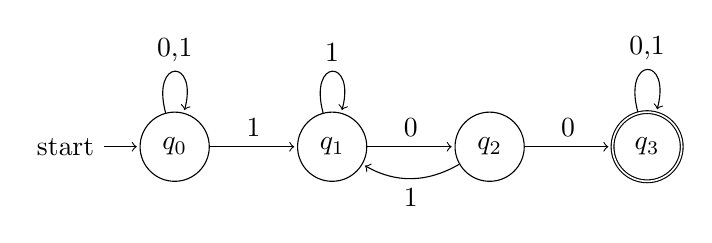
\begin{tikzpicture}[shorten >=1pt,node distance=2cm,on grid,auto]
  \node[state, initial] (q0) {$q_0$};
  \node[state] (q1) [right=of q0] {$q_1$};
  \node[state] (q2) [right=of q1] {$q_2$};
  \node[state, accepting] (q3) [right=of q2] {$q_3$};

  \path[->] 
    (q0) edge [loop above] node {0,1} ()
         edge node {1} (q1)
    (q1) edge [loop above] node {1} ()
         edge node {0} (q2)
    (q2) edge [bend left] node {1} (q1)
         edge node {0} (q3)
    (q3) edge [loop above] node {0,1} ();
\end{tikzpicture}
\end{center}

\textbf{1. Language Description:}  
The NFA accepts all strings containing the substring \texttt{100}. Once this pattern is seen, the automaton reaches $q_3$ (an accepting state), which loops on any input. Thus, 
\[
L(A) = \{ w \in \{0,1\}^* \mid w \text{ contains the substring } 100 \}
\]

\textbf{2. Formal Definition:}
\[
\begin{aligned}
Q &= \{q_0, q_1, q_2, q_3\}, \quad \Sigma = \{0,1\} \\
\delta(q_0, 0) &= \{q_0\}, \quad \delta(q_0, 1) = \{q_0, q_1\} \\
\delta(q_1, 0) &= \{q_2\}, \quad \delta(q_1, 1) = \{q_1\} \\
\delta(q_2, 0) &= \{q_3\}, \quad \delta(q_2, 1) = \{q_1\} \\
\delta(q_3, 0) &= \{q_3\}, \quad \delta(q_3, 1) = \{q_3\} \\
q_0 &= q_0, \quad F = \{q_3\}
\end{aligned}
\]

\textbf{3. Extended Transition:}  
Compute $\hat{\delta}(q_0, 10110)$ step-by-step:
\[
\begin{aligned}
\hat{\delta}(q_0, 1) &= \{q_0, q_1\} \\
\hat{\delta}(\{q_0, q_1\}, 0) &= \delta(q_0, 0) \cup \delta(q_1, 0) = \{q_0, q_2\} \\
\hat{\delta}(\{q_0, q_2\}, 1) &= \delta(q_0,1) \cup \delta(q_2,1) = \{q_0, q_1\} \\
\hat{\delta}(\{q_0, q_1\}, 1) &= \{q_0, q_1\} \\
\hat{\delta}(\{q_0, q_1\}, 0) &= \{q_0, q_2\}
\end{aligned}
\]
Final state: $\{q_0, q_2\}$

\textbf{4. Paths for $v = 1100$ and $w = 1010$:}
\begin{itemize}
\item $v = 1100$: Final state includes $q_3$ $\Rightarrow$ Accepted
\item $w = 1010$: Final state does not include $q_3$ $\Rightarrow$ Not accepted
\end{itemize}

\textbf{5. Power Set Construction (DFA $A_D$):}
Use subset construction:
\[
\begin{aligned}
\text{Start: } & \{q_0\} \\
\delta_D(\{q_0\}, 1) &= \{q_0, q_1\} \\
\delta_D(\{q_0, q_1\}, 0) &= \{q_0, q_2\} \\
\delta_D(\{q_0, q_2\}, 0) &= \{q_0, q_3\}, \text{ etc.}
\end{aligned}
\]
Accepting subsets are any that include $q_3$.

\textbf{6. Language Verification:}  
By construction, $L(A_D) = L(A)$.

\textbf{7. DFA Minimization:}  
Yes, a smaller DFA exists. The minimal DFA recognizing $\{ w \mid w \text{ contains } 100 \}$ has 4 states tracking whether `1`, `10`, and `100` have been seen.


\subsubsection{Exploration}

This material helps bridge the gap between formal theory and real-world tools. It shows how concepts like regular expressions, which are common in programming and data processing, are deeply connected to theoretical models like automata. Learning this gives us a better understanding of how programs recognize patterns in text and how tools like compilers or search systems are built. Regular expressions give us a way to describe patterns simply, while automata provide a precise model to execute those patterns.


\subsubsection{Questions}

Why do we use regular expressions in practice instead of DFAs, even though both can describe the same languages?

\subsection{Week 5}

\subsubsection{Notes}

Chapter 4 introduces several important concepts related to regular languages. One of the most powerful tools is the Pumping Lemma, which helps prove that certain languages are not regular by showing that long enough strings in the language must have a repeatable middle part. If repeating that part leads to a string not in the language, then the language can't be regular. The chapter also covers many operations that keep languages regular, such as union, concatenation, closure (using the star operation), intersection, complementation, difference, reversal, and even symbol-to-string replacements (homomorphisms). There are also algorithms to check whether a regular language is empty, or whether a specific string belongs to it. Another major topic is distinguishing states in a DFA. Two states are distinguishable if some input causes one to lead to an accepting state while the other does not. By identifying all such differences, we can simplify the DFA by combining states that behave the same. This leads to DFA minimization, which gives the smallest possible version of a machine that still recognizes the same language.

\subsubsection{Homework}

\textbf{Exercise 3.2.1 – From DFA to Regular Expressions}

We are given a DFA with the following transition table:

\begin{center}
\begin{tabular}{c|cc}
      & 0   & 1   \\
\hline
$\rightarrow q_1$ & $q_2$ & $q_1$ \\
$q_2$             & $q_3$ & $q_1$ \\
$*q_3$            & $q_3$ & $q_2$ \\
\end{tabular}
\end{center}

\textbf{(a) Regular expressions $R_{ij}^{(0)}$} (direct transitions only):

\begin{center}
\begin{tabular}{c|ccc}
$i \rightarrow j$ & 1 & 2 & 3 \\
\hline
1 & 1 & 0 & $\emptyset$ \\
2 & 1 & $\emptyset$ & 0 \\
3 & $\emptyset$ & 1 & 0 \\
\end{tabular}
\end{center}

\textbf{(b) Regular expressions $R_{ij}^{(1)}$} (paths through $q_1$ allowed):

\[
\begin{aligned}
R_{11}^{(1)} &= 1 + 1(1)^*1 = 1(1)^* \\
R_{12}^{(1)} &= 0 + 1(1)^*0 = 1(1)^*0 \\
R_{13}^{(1)} &= \emptyset \\
R_{21}^{(1)} &= 1 \\
R_{22}^{(1)} &= \emptyset \\
R_{23}^{(1)} &= 0 \\
R_{31}^{(1)} &= \emptyset \\
R_{32}^{(1)} &= 1 \\
R_{33}^{(1)} &= 0 \\
\end{aligned}
\]

\textbf{(c) Regular expressions $R_{ij}^{(2)}$} (paths through $q_1$ and $q_2$ allowed):

\[
\begin{aligned}
R_{11}^{(2)} &= 1(1)^* + 1(1)^*0 (\emptyset)^* 1 = 1(1)^* \\
R_{12}^{(2)} &= 1(1)^*0 \\
R_{13}^{(2)} &= \emptyset + 1(1)^*0 (\emptyset)^* 0 = 1(1)^*00 \\
R_{21}^{(2)} &= 1 \\
R_{22}^{(2)} &= \emptyset \\
R_{23}^{(2)} &= 0 \\
R_{31}^{(2)} &= 1 \\
R_{32}^{(2)} &= 1 \\
R_{33}^{(2)} &= 0 \\
\end{aligned}
\]

\textbf{(d) Regular expression for the language of the automaton:}

We start at $q_1$ and the accepting state is $q_3$, so we are interested in $R_{13}^{(3)}$. Since $R_{22}^{(2)} = \emptyset$, we have:

\[
R_{13}^{(3)} = R_{13}^{(2)} + R_{12}^{(2)} (\emptyset)^* R_{23}^{(2)} = 1(1)^*00
\]

\textbf{Conclusion:} The regular expression for the language accepted by the DFA is:
\[
\boxed{1(1)^*00}
\]

This describes the set of strings that contain one or more 1s followed by two 0s.

\textbf{Exercise 3.2.2 – Regular Expression from DFA}

We are given the following DFA:

\begin{center}
\begin{tabular}{c|cc}
      & 0   & 1   \\
\hline
$\rightarrow q_1$ & $q_2$ & $q_3$ \\
$q_2$             & $q_1$ & $q_3$ \\
$*q_3$            & $q_2$ & $q_1$ \\
\end{tabular}
\end{center}

\textbf{(c) Regular expressions $R_{ij}^{(2)}$}

Using the direct transitions and paths through $q_1$ and $q_2$, we focus on computing the expression from $q_1$ to $q_3$, denoted $R_{13}^{(2)}$:

\[
R_{13}^{(2)} = 1 + 0(0)^*1
\]

This expression accounts for:
\begin{itemize}
    \item A direct transition from $q_1$ to $q_3$ via input $1$
    \item An indirect path through $q_2$ via $0$, possibly looping on $q_2$ with $0$s, and ending in $1$
\end{itemize}

\textbf{(d) Regular expression for the language of the automaton}

Since the start state is $q_1$ and the accepting state is $q_3$, the expression from $q_1$ to $q_3$ represents the language accepted by this DFA. Therefore, the regular expression for the language is:

\[
\boxed{1 + 0(0)^*1}
\]

This describes strings that either:
\begin{itemize}
    \item Begin with a 1 (direct path), or
    \item Begin with a 0, followed by any number of 0s, and then a 1
\end{itemize}

\textbf{Exercise 4.4.1 – Minimizing the DFA of Figure 4.14}

\textbf{(a) Table of Distinguishabilities:}

The DFA has states $\{A, B, C, D, E, F, G, H\}$, with $D$ as the only accepting state.

We use the table-filling method:
\begin{itemize}
    \item Step 1: Mark all pairs where one state is accepting and the other is not:
    \[
    \{AD, BD, CD, DE, DF, DG, DH\}
    \]
    \item Step 2: Iteratively mark pairs whose transitions lead to already marked pairs. For example:
    \begin{itemize}
      \item \( AE(0) = B, D \Rightarrow BD \text{ is marked} \Rightarrow \text{mark } AE \)
      \item \( AF(0) = B, D \Rightarrow BD \text{ is marked} \Rightarrow \text{mark } AF \)
      \item \( AH(1) = A, D \Rightarrow AD \text{ is marked} \Rightarrow \text{mark } AH \)
    \end{itemize}
  
    \item After finishing the process, the indistinguishable state groups are:
    \[
    \{A, C\}, \quad \{B, F, G, H\}, \quad \{D\}
    \]
\end{itemize}

\textbf{(b) Constructing the Minimum-State DFA:}

\begin{itemize}
    \item Group equivalent states:
    \[
    [A,C], [B,F,G,H], [D]
    \]
    \item Transition table (using representatives):
\end{itemize}

\begin{center}
\begin{tabular}{c|c|c}
State & 0 & 1 \\
\hline
$[A,C]$ & $[B,F,G,H]$ & $[A,C]$ \\
$[B,F,G,H]$ & $[B,F,G,H]$ & $[A,C]$ \\
$[D]$ & $[D]$ & $[A,C]$ \\
\end{tabular}
\end{center}

\begin{itemize}
    \item Start state: $[A,C]$
    \item Accepting state: $[D]$
\end{itemize}

\vspace{1em}
\textbf{Exercise 4.4.2 – Minimizing the DFA of Figure 4.15}

\textbf{(a) Table of Distinguishabilities:}

States: $\{A, B, C, D, E, F, G, H, I\}$  
Accepting states: $\{C, F, I\}$

\begin{itemize}
    \item Mark pairs with one accepting and one non-accepting state:
    \[
    \text{All combinations of } \{C, F, I\} \text{ with } \{A, B, D, E, G, H\}
    \]
    \item Apply transitions and iteratively mark new pairs. The final equivalent classes are:
    \[
    \{A, H\}, \quad \{B\}, \quad \{C, I\}, \quad \{D, E\}, \quad \{F\}, \quad \{G\}
    \]
\end{itemize}

\textbf{(b) Constructing the Minimum-State DFA:}

\begin{itemize}
    \item Equivalence classes:
    \[
    [A,H], [B], [C,I], [D,E], [F], [G]
    \]
    \item Transition table (representatives used):
\end{itemize}

\begin{center}
\begin{tabular}{c|c|c}
State & 0 & 1 \\
\hline
$[A,H]$ & $[B]$ & $[D,E]$ \\
$[B]$   & $[C,I]$ & $[F]$ \\
$[C,I]$ & $[D,E]$ & $[A,H]$ \\
$[D,E]$ & $[F]$ & $[G]$ \\
$[F]$   & $[G]$ & $[B]$ \\
$[G]$   & $[A,H]$ & $[C,I]$ \\
\end{tabular}
\end{center}

\begin{itemize}
    \item Start state: $[A,H]$
    \item Accepting states: $[C,I], [F]$
\end{itemize}


\subsubsection{Exploration}

This chapter connects practical techniques with deeper ideas in computer science. The Pumping Lemma is theoretical but very powerful — it gives a strategy to prove limitations of regular languages. On the other hand, operations like union and complementation show that regular languages are very flexible and stable under transformation. DFA minimization not only helps simplify machines but also gives insight into the essential structure of a language. These concepts show up in compiler design, formal verification, and string processing tools.

\subsubsection{Questions}

Why is it helpful to make a DFA smaller, and how do we know which states we can combine?

\subsection{Week 6 and 7}

\subsubsection{Notes}

These sections introduce the limits of what computers can do. Section 8.1 uses simple C programs, like one that prints “hello, world,” to illustrate how some problems can’t be solved by any program — these are called undecidable problems. Section 8.2 introduces Turing machines, simple abstract models of computation that let us reason more clearly about what is computable. In Section 9.1, we see that some languages, like the diagonalization language, are not even recursively enumerable — meaning no Turing machine can accept them. Section 9.2 explains the difference between RE and decidable languages: RE languages can be accepted by a Turing machine, but it may run forever if the input isn’t in the language. Decidable languages are those where the machine always halts.



\subsubsection{Homework}

\textbf{Exercise 1 – Language Classification (Simplified)}

\begin{itemize}
    \item \textbf{$L_1 = \{ M \mid M \text{ halts on input } M \}$} \\
    Recursively enumerable (not decidable, not co-r.e.)

    \item \textbf{$L_2 = \{ (M, w) \mid M \text{ halts on input } w \}$} \\
    Recursively enumerable (not decidable, not co-r.e.)

    \item \textbf{$L_3 = \{ (M, w, k) \mid M \text{ halts on } w \text{ in at most } k \text{ steps} \}$} \\
    Decidable (also r.e. and co-r.e.)
\end{itemize}

\vspace{1em}
\textbf{Exercise 2 – Logical Properties of Language Classes (Simplified but Explained)}

\begin{itemize}
    \item \textbf{If $L_1$ and $L_2$ are decidable, then $L_1 \cup L_2$ is decidable.} \\
    \textit{True.} Run both deciders on the input. If either accepts, accept.

    \item \textbf{If $L$ is decidable, then $\overline{L}$ is decidable.} \\
    \textit{True.} A decider for $L$ always halts, so we can flip the result to decide its complement.

    \item \textbf{If $L$ is decidable, then $L^*$ is decidable.} \\
    \textit{True.} We can try all ways of splitting the input into substrings and check if each part is in $L$ using its decider.

    \item \textbf{If $L_1$ and $L_2$ are r.e., then $L_1 \cup L_2$ is r.e.} \\
    \textit{True.} We can simulate both recognizers in parallel and accept if either one does.

    \item \textbf{If $L$ is r.e., then $\overline{L}$ is r.e.} \\
    \textit{False.} The Halting Problem is r.e., but its complement is not, since we cannot always confirm non-halting.

    \item \textbf{If $L$ is r.e., then $L^*$ is r.e.} \\
    \textit{True.} We can non-deterministically try decompositions of the input and use the recognizer for $L$ on each piece.
\end{itemize}



\subsubsection{Exploration}

Understanding the limits of computation is essential in both theory and practice. Knowing which problems are undecidable or only semi-decidable (RE) helps programmers avoid wasting time trying to fully solve problems that are impossible to decide. These ideas also help frame deeper questions in computer science, logic, and software design.



\subsubsection{Questions}

Why do some RE languages have no halting procedure, even though they’re accepted by a Turing machine?

\subsection{Week 8 and 9}

\subsubsection{Notes}

Sections 10.1–10.3 introduce the theory of intractability, focusing on problems that are solvable in principle but likely not in practice due to their high time complexity. A key distinction is made between the classes P (problems solvable in polynomial time by a deterministic Turing machine) and NP (problems verifiable in polynomial time by a nondeterministic Turing machine). The concept of NP-completeness is introduced to identify the "hardest" problems in NP, with SAT (Boolean satisfiability) being the first proven NP-complete problem, via Cook’s Theorem. The theory emphasizes the importance of polynomial-time reductions, which let us show that solving one hard problem efficiently would enable us to solve all NP problems efficiently. Section 10.3 narrows in on 3SAT, a more structured version of SAT, which makes it easier to use in reductions to other NP-complete problems. Despite its restricted form, 3SAT remains NP-complete and plays a central role in complexity theory.

\subsubsection{Homework}

\textbf{Exercise 1 – Order of Growth}

Order the following functions from slowest to fastest growth:

\[
\log(\log n), \quad \log n, \quad e^{\log n} = n, \quad e^{2\log n} = n^2, \quad 2^n, \quad n!, \quad 2^{2^n}
\]

Answer:
\[
\log(\log n) < \log n < n < n^2 < 2^n < n! < 2^{2^n}
\]

\vspace{1em}

\textbf{Exercise 2 – Big O Properties}

Let \( f, g, h : \mathbb{N} \rightarrow \mathbb{R}_{\geq 0} \). Show the following:

\begin{itemize}
    \item \( f \in O(f) \) \\
    Let \( M = 1 \), \( N = 1 \). Then for all \( n \geq N \), \( f(n) \leq M \cdot f(n) \).

    \item \( O(c \cdot f) = O(f) \), for constant \( c > 0 \) \\
    A constant factor does not change the asymptotic growth, as it can be absorbed into the Big O constant.

    \item If \( f(n) \leq g(n) \) for large \( n \), then \( O(f) \subseteq O(g) \) \\
    If \( f(n) \leq g(n) \), then anything bounding \( g(n) \) will also bound \( f(n) \).

    \item If \( O(f) \subseteq O(g) \), then \( O(f + h) \subseteq O(g + h) \) \\
    Adding the same function \( h(n) \) to both does not affect the relative growth rate.

    \item If \( h(n) > 0 \) and \( O(f) \subseteq O(g) \), then \( O(f \cdot h) \subseteq O(g \cdot h) \) \\
    Multiplying both functions by a positive function \( h(n) \) preserves the inequality.
\end{itemize}

\vspace{1em}

\textbf{Exercise 3 – Polynomial Bounds}

\begin{itemize}
    \item If \( j \leq k \), then \( O(n^j) \subseteq O(n^k) \) \\
    For large \( n \), \( n^j \leq n^k \), so this holds.

    \item If \( j \leq k \), then \( O(n^j + n^k) \subseteq O(n^k) \) \\
    The higher-degree term dominates for large \( n \), so the sum is in \( O(n^k) \).

    \item \( O\left(\sum_{i=0}^{k} a_i n^i\right) = O(n^k) \) \\
    A polynomial is dominated by its highest-degree term asymptotically.

    \item \( O(\log n) \subseteq O(n) \) \\
    Since \( \log n \leq n \), this inclusion is valid.

    \item \( O(n \log n) \subseteq O(n^2) \) \\
    As \( \log n \leq n \), then \( n \log n \leq n^2 \), so this is true.
\end{itemize}


\subsubsection{Exploration}

This chapter shifts our focus from asking whether a problem can be solved to whether it can be solved efficiently. It introduces the idea that some problems, although technically solvable, might take an unrealistic amount of time to compute as their inputs grow. This is extremely relevant in real life, where fast solutions are critical in areas like data encryption, logistics, and software performance.

A key idea is the difference between checking a solution and actually finding one. Some problems are easy to verify but hard to solve — a concept at the heart of the debate over whether "P" equals "NP." The chapter also introduces the idea of reducing one problem to another in a way that preserves difficulty. If you can show a hard problem transforms into another problem efficiently, it means the second problem is also hard.

The concept of 3SAT, a structured version of the satisfiability problem, shows how even simple-looking restrictions can still represent highly complex problems. Understanding these reductions helps us organize problems into complexity classes and reason about what might or might not be possible in computing.
\subsubsection{Questions}

How can a more structured version of a problem, like 3SAT, be just as hard as the general version (SAT)?

\subsection{Week 10 and 11}

\subsubsection{Notes}

Chapters 10.1 and 10.2 explore the idea of efficient computation. The main goal is to separate problems that can be solved quickly from those that cannot. Problems in the class P can be solved by a standard algorithm in polynomial time. Problems in NP may not be easy to solve, but if someone gives you a solution, you can check it quickly.

The chapter introduces nondeterministic Turing machines as a way to understand problems in NP. It also explains the idea of polynomial-time reductions. These reductions help us compare problems by showing how solving one would help solve another. Cook’s Theorem shows that the SAT problem is the first known NP-complete problem. This means it is at least as hard as every other problem in NP.

\subsubsection{Homework}

\textbf{Exercise 1 – Convert to CNF}

\begin{itemize}
    \item \(\varphi_1 := \neg((a \land b) \lor (\neg c \land d))\)

    Apply De Morgan's laws:
    \[
    \neg((a \land b) \lor (\neg c \land d)) \equiv (\neg a \lor \neg b) \land (c \lor \neg d)
    \]

    \item \(\varphi_2 := \neg((p \lor q) \rightarrow (r \land \neg s))\)

    First rewrite implication:
    \[
    (p \lor q) \rightarrow (r \land \neg s) \equiv \neg(p \lor q) \lor (r \land \neg s)
    \]

    Then apply De Morgan:
    \[
    \neg[\neg(p \lor q) \lor (r \land \neg s)] \equiv (p \lor q) \land (\neg r \lor s)
    \]
\end{itemize}

\vspace{1em}
\textbf{Exercise 2 – Satisfiability}

\begin{itemize}
    \item \(\psi_1 := (a \lor \neg b) \land (\neg a \lor b) \land (\neg a \lor \neg b)\)

    Let \(a = \text{false}, b = \text{false}\). All three clauses evaluate to true.

    \textbf{Answer:} Satisfiable. One assignment is \(a = \text{false}, b = \text{false}\).

    \item \(\psi_2 := (\neg p \lor q) \land (\neg q \lor r) \land \neg(\neg p \lor r)\)

    The third clause becomes \(p \land \neg r\), so the formula becomes:
    \[
    (\neg p \lor q) \land (\neg q \lor r) \land p \land \neg r
    \]
    Let \(p = \text{true}, r = \text{false}\). Then \(q\) must be true (clause 1), but then clause 2 fails.

    \textbf{Answer:} Unsatisfiable. No assignment satisfies all clauses.

    \item \(\psi_3 := (x \lor y) \land (\neg x \lor y) \land (x \lor \neg y) \land (\neg x \lor \neg y)\)

    Test all four combinations of truth values. None satisfy all clauses.

    \textbf{Answer:} Unsatisfiable.
\end{itemize}

\vspace{1em}
\textbf{Exercise 3 – Sudoku Encoding (CNF)}

Let \(x_{r,c,v}\) be a variable that is true iff cell \((r, c)\) contains value \(v\), with \(r, c, v \in \{1, \dots, 9\}\).

\begin{itemize}
    \item \(\mathbf{C_1}\): Each cell has at least one value
    \[
    \bigwedge_{r=1}^{9} \bigwedge_{c=1}^{9} \left( \bigvee_{v=1}^{9} x_{r,c,v} \right)
    \]

    \item \(\mathbf{C_2}\): Each cell has at most one value
    \[
    \bigwedge_{r=1}^{9} \bigwedge_{c=1}^{9} \bigwedge_{1 \leq v < w \leq 9} (\neg x_{r,c,v} \lor \neg x_{r,c,w})
    \]

    \item \(\mathbf{C_3}\): Each row contains all digits
    \[
    \bigwedge_{r=1}^{9} \bigwedge_{v=1}^{9} \left( \bigvee_{c=1}^{9} x_{r,c,v} \right)
    \]

    \item \(\mathbf{C_4}\): Each column contains all digits
    \[
    \bigwedge_{c=1}^{9} \bigwedge_{v=1}^{9} \left( \bigvee_{r=1}^{9} x_{r,c,v} \right)
    \]

    \item \(\mathbf{C_5}\): Each \(3 \times 3\) block contains all digits

    Let \(i, j \in \{0, 1, 2\}\) be block indices:
    \[
    \bigwedge_{v=1}^{9} \bigwedge_{i=0}^{2} \bigwedge_{j=0}^{2} \left( \bigvee_{r=1}^{3} \bigvee_{c=1}^{3} x_{3i + r, 3j + c, v} \right)
    \]

    \item \(\mathbf{C_6}\): Given clues

    For each clue stating cell \((r,c)\) has value \(v\), include:
    \[
    x_{r,c,v}
    \]
\end{itemize}


\subsubsection{Exploration}

It is helpful to think of this topic in terms of checking versus solving. Some problems are hard to solve, but once you have a solution, checking it is easy. This shows how P and NP differ. The chapter also highlights how reductions help researchers figure out if new problems are related to older, well-understood problems.

These ideas are not just theoretical. In areas like cryptography, scheduling, and artificial intelligence, understanding whether a problem is in P or NP affects how software is designed. If we believe that P is not equal to NP, then we focus on creating better approximations or faster checks rather than trying to solve every case directly.

\subsubsection{Questions}

What makes NP-complete problems so important in both theory and practice?

\subsection{Week 12 and 13}

\subsubsection{Notes}

Sections 14.1 to 14.4 focus on using graph theory to solve flow problems in transport networks. These networks are modeled as directed graphs with edge capacities, and the goal is to maximize flow or minimize cost. The max-flow min-cut theorem is central: the maximum flow equals the capacity of the smallest cut between source and sink.

Extensions include handling multiple sources and sinks by adding a supersource and supersink with unlimited capacity edges. Cost optimization involves finding least-cost paths and updating capacities after each flow. Multicommodity flow introduces multiple goods with their own sources and sinks, sharing edge capacities and maintaining flow conservation.

\subsubsection{Homework}

\textbf{Exercise 1: Maximal Flow and Minimal Cut}\\
We apply the Ford-Fulkerson algorithm to the given flow network to compute a maximal flow and determine a minimal cut.\\

\textbf{Step 1: Initialize Flow}\\
Initially, all flow values on the edges are set to 0.

\textbf{Step 2: Augmenting Paths Using Ford-Fulkerson}\\
We search for augmenting paths from $s$ to $t$ with available capacity:

\begin{itemize}
    \item \textbf{First Augmenting Path:} $s \rightarrow a \rightarrow d \rightarrow t$\\
    Bottleneck capacity: $\min(10 - 8, 8 - 0, 10 - 8) = 2$\\
    Add 2 units of flow.

    \item \textbf{Second Augmenting Path:} $s \rightarrow b \rightarrow d \rightarrow t$\\
    Bottleneck capacity: $\min(10 - 0, 9 - 0, 10 - 8) = 2$\\
    Add 2 units of flow.

    \item \textbf{Third Augmenting Path:} All paths from $s$ to $t$ are either blocked or saturated. No more augmenting paths exist.
\end{itemize}

\textbf{Step 3: Final Flow}\\
Total flow from source $s$ is:
\[\text{Flow}(s) = \text{flow}(s \rightarrow a) + \text{flow}(s \rightarrow b) = 8 + 2 = 10\]
Thus, the \textbf{maximum flow} is \textbf{10}.

\textbf{Step 4: Minimal Cut}\\
To find a minimal cut, we examine the residual graph after the algorithm terminates. The reachable vertices from $s$ are $\{s, a, b\}$, and the remaining vertices are $\{c, d, t\}$.

Edges crossing from $S = \{s, a, b\}$ to $T = \{c, d, t\}$ are:
\begin{itemize}
    \item $a \rightarrow c$ with capacity 4
    \item $b \rightarrow d$ with capacity 9
\end{itemize}
Total capacity of these edges = $4 + 6 = 10$. Hence, the \textbf{minimal cut} has capacity \textbf{10}, which matches the maximum flow.

\textbf{Step 5: Uniqueness of Maximal Flow}\\
The maximal flow is \textbf{not necessarily unique}. Different paths and flow assignments can yield the same total flow value but distribute the flow across edges differently.


\subsubsection{Exploration}

These sections show how graph models simplify complex transport and logistics problems. Using artificial nodes to unify multi-source problems is clever and practical. Multicommodity flow problems highlight real-world challenges in resource sharing and prioritization.

\subsubsection{Questions}

What strategies can ensure fair flow distribution in multicommodity networks?



\section{Connecting the Dots: From Theory to Practice}

The study of algorithms and computation is often viewed as abstract and disconnected from the reality of software development and problem-solving. However, through the exploration of automata theory, formal languages, Turing machines, and algorithmic complexity, I have come to appreciate how foundational these concepts are to practical computing. This synthesis reflects on that journey and highlights how theoretical principles underpin everyday technologies.

A key realization came when studying finite automata and regular languages. Initially, the transition diagrams and formal definitions seemed like puzzles with limited real-world application. But as we progressed into topics like lexical analysis in compilers, it became clear that finite automata directly model the way programming languages process syntax. This connection between theoretical models and software tools is profound: regular expressions, for example, are a direct application of regular languages in text processing and searching algorithms.

The concept of decidability marked another pivotal point. Learning about the halting problem and the class of recursively enumerable languages not only clarified the boundaries of computation but also influenced my understanding of why certain software bugs are fundamentally undecidable. Alan Turing's formulation of the Turing machine as a universal model of computation gave me a lens through which to view any algorithm, not just as code but as a formal process with limitations and guarantees~\cite{turing1937}.

When we encountered the P vs. NP problem, the relevance of computational complexity became personal. I began to notice that the runtime behavior of programs I wrote in other classes echoed the complexity classes we studied. Simple brute-force search methods felt inefficient not just in execution time but in principle. The discussions of polynomial-time reductions and NP-completeness provided a formal way to understand why some problems in scheduling, optimization, and game theory resist efficient solutions.

This theory-practice connection has deepened my respect for algorithm design. What once seemed like arbitrary constraints in software---timeouts, approximation algorithms, or limits on input size---are now visible as practical reflections of underlying complexity barriers. Moreover, theoretical insights have practical consequences. For example, understanding why SAT is NP-complete explains the existence and limitations of SAT solvers, which are widely used in fields ranging from software verification to artificial intelligence~\cite{cook1971}.

The synthesis of this course material has changed the way I think about computing. I now approach problems with a deeper analytical mindset, often framing them in terms of automata, reductions, and complexity. Rather than seeing theory as separate from practice, I see it as a necessary foundation that informs how and why we build the systems we do.


\section{Evidence of Participation}

Engineering Seminar -- Prof. Lorenzo Mangolini on Plasma Science

On Monday, I attended a seminar at the Fowler School of Engineering hosted by Prof. Lorenzo Mangolini from UC Riverside. The talk centered on plasma science and its practical applications across industries, particularly in materials engineering and nanotechnology. Prof. Mangolini began by explaining what plasma is---often referred to as the ``fourth state of matter''---and how it is used to modify the surface properties of materials in ways that are otherwise difficult to achieve through conventional methods.

A major focus of the seminar was on the use of low-temperature plasmas to engineer advanced materials for electronics and energy storage devices. He discussed how plasma-assisted processes can reduce manufacturing time and environmental impact, especially in the production of thin films and carbon-based nanomaterials. The seminar also touched on interdisciplinary collaborations between physicists, chemists, and engineers to advance the field.

What I found particularly interesting was the emphasis on scalability and how some of the lab-scale innovations in plasma processing are being transitioned into industrial applications. Prof. Mangolini’s examples illustrated the challenges and promises of bridging fundamental science and real-world engineering.

\textbf{My Question:} How do plasma processing techniques compare to traditional methods in terms of long-term reliability and material degradation under everyday usage?

\section{Conclusion}\label{conclusion}

This course offered a unique opportunity to step back from the fast-paced world of application development and investigate the foundational theories that underpin modern computing. Through the lens of automata theory, Turing machines, complexity theory, and undecidability, I gained not only technical knowledge but also a broader understanding of what is possible—and what is impossible—within software systems. This perspective is vital for any software engineer aiming to write robust, scalable, and meaningful code in a world increasingly dependent on algorithmic decision-making.

What stood out to me most was the dual nature of computing: the balance between elegance and limitation. On one hand, concepts like finite automata and regular expressions provide clean, formal models that translate directly into everyday tools such as compilers, text search, and pattern matching. On the other hand, the study of undecidable problems and complexity classes like NP reminds us that no matter how powerful our machines become, certain problems will remain intractable or uncomputable. Recognizing these boundaries helped me understand the real value of heuristics, approximations, and modular design in practical software engineering.

Another key takeaway is the importance of abstraction and modeling. Learning to view problems through the lens of state machines or computational classes forces a mindset shift that is deeply valuable in both systems design and algorithmic thinking. It encourages clarity, precision, and a structured approach to tackling complexity.

In terms of improvements, I would suggest integrating more project-based assessments that allow students to apply theoretical concepts to real-world contexts—perhaps through building simplified versions of lexical analyzers, designing custom decision procedures, or working with constraint solvers. Additionally, increased use of interactive tools like Turing machine simulators, automata visualizers, or complexity experiment sandboxes could make the learning process more tangible.

Ultimately, this course helped demystify the theoretical core of computer science and revealed its ongoing relevance in the daily work of software engineers. Rather than seeing theory and practice as separate domains, I now view them as interdependent. Theoretical models clarify the limits and capabilities of software, while practice brings those models to life through implementation. I leave the course with a deeper respect for both.

\begin{thebibliography}{99}
  \bibitem{cook1971} Stephen A. Cook, \emph{The Complexity of Theorem-Proving Procedures}, Proceedings of the Third Annual ACM Symposium on Theory of Computing, 1971. \url{https://doi.org/10.1145/800157.805047}
  \bibitem{turing1937} Alan M. Turing, \emph{On Computable Numbers, with an Application to the Entscheidungsproblem}, Proceedings of the London Mathematical Society, 1937. \url{https://doi.org/10.1112/plms/s2-42.1.230}
  \end{thebibliography}

\end{document}
